\section{Validação de projeto}
\label{sec:validacao}

Nessa seção será discutido como a simulação deve ser
realizada para validação dos requisitos de projeto, assim como a configuração do
ambiente virtual submarino.

\subsection{Módulos de simulação}
\label{sec:simu-modules}

A simulação fidedigna de um veículo submarino deve contar com a simulação dos
atuadores, sensores e da física de corpo rígido debaixo d'água. Com o objetivo de obter uma simulação que incluísse todos esses tópicos, algumas soluções de \textit{software} disponíveis serão adotas e algumas desenvolvidas, como está descrito a seguir.

\subsubsection*{Sensores, atuadores e física}

A função de simular o comportamento de um robô no meio com seus sensores e
atuadores é tarefa de um simulador de robótica. A Tabela \ref{tab:simulators-comparison} mostra as alternativas de simuladores
que possuem funcionalidades essenciais para validação de um robô submarino.
Dentre as cinco alternativas apresentadas, três delas utilizam o simulador Gazebo \cite{gazebo}: UWSim (do inglês {\it Underwater Simulator}), UUV
(do inglês {\it Unmanned Underwater Vehicle Simulator}) e USVSim (do inglês {\it Unmanned Surface
Vehicle Simulator}). Dentre esses, o USVSim é o mais completo, pois dispõe
de quase todas as funcionalidades analisadas.

\begin{table}[h]
    \label{tab:simulators-comparison}
    \caption{Tabela comparativa de simuladores e suas funcionalidades}
    \centering
    \includegraphics[width=1\textwidth]{images/simulators_comparison.png}\\
    \footnotesize Fonte: \cite{simulators-comparison}
\end{table}

Recentemente, a Open Robotic lançou o Ignition, um novo simulador de robótica que substituirá o Gazebo. Pelo fato desse simulador incorporar todas as funcionalidades descritas na Tabela \ref{tab:simulators-comparison}, ele foi selecionado para ser o \textit{software} de simulação. Ademais, no Ignition é possível carregar um ambiente submarino 3D e o veículo, sendo possível visualizar, mas também obter dados simulados de sensores, controlar motores e simular a interação do robô com o ambiente ao seu redor.

\subsubsection*{Comunicação}
Apesar do Ignition possibilitar a simulação dos motores e sensores do veículo, a simulação da comunicação por meio sensor acústico é uma funcionalidade que não consta no \textit{software}. Portanto, serão desenvolvidos \textit{plugins} para o \textit{software} que simulam as peculiaridades desse tipo de sensor. Os \textit{plugins} devem simular atraso da onda sonora na água, ruído e atenuação.

Para simular a comunicação, foi escolhida preliminarmente a biblioteca AUVNetSim \cite{montana2008auvnetsim}, que contém uma grande variedade parâmetros e protocolos para redes acústicas subaquáticas. Na simulação de cada nó acústico nessa biblioteca, a comunicação é realizada por troca de mensagens curtas entre as camadas que podem ser configuradas na ordem descrita na Figura \ref{fig:auvnetsim}.

\begin{figure}[h]
	\centering
	\caption{Estrutura de programação de um nó acústico AUVNetSim}
	\label{fig:auvnetsim}
	\includegraphics[width=0.3\linewidth]{images/auvnetsim}\\
	\footnotesize Fonte: \cite{montana2008auvnetsim}
\end{figure}

Outros ferramentas disponíveis no mercado fornecem mais funcionalidades do que a AUVNetSim, como a Network Simulator (NS-3), a SUNSET ou a Aqua-Sim \cite{godi2021survey}. Contudo, AUVNetSim foi selecionada por ser de código aberto, possuir manual de utilização e ser de fácil integração e manutenção \cite{montana2008auvnetsim}.

De forma a simular a comunicação com o protótipo, a AUVNetSim será integrada com o \textit{framwork} ROS (do inglês \textit{Robot Operating System}). Do mesmo modo, ainda serão estudados, avaliados e testados outros protocolos propostos na literatura com o propósito de se obter uma configuração satisfatória e que se aproxime do mundo real na simulação.

\subsection{Missões}

\subsubsection*{Submersão e emersão controlada}
Essa missão consiste em submergir e emergir o ROV a uma determinada profundidade,
como pode ser visto na Figura \ref{fig:descenttest} Esse procedimento será executado tanto com controle manual de velocidade, como também com controle automático, no qual o ROV se desloca ao longo de um caminho previamente estabelecido. Além disso, Arucos serão posicionados ao longo de todo o trajeto para obtenção de uma medição mais precisa de profundidade.


\begin{figure}[h]
	\centering
	\caption{Missão de submersão e emersão}
	\label{fig:descenttest}
	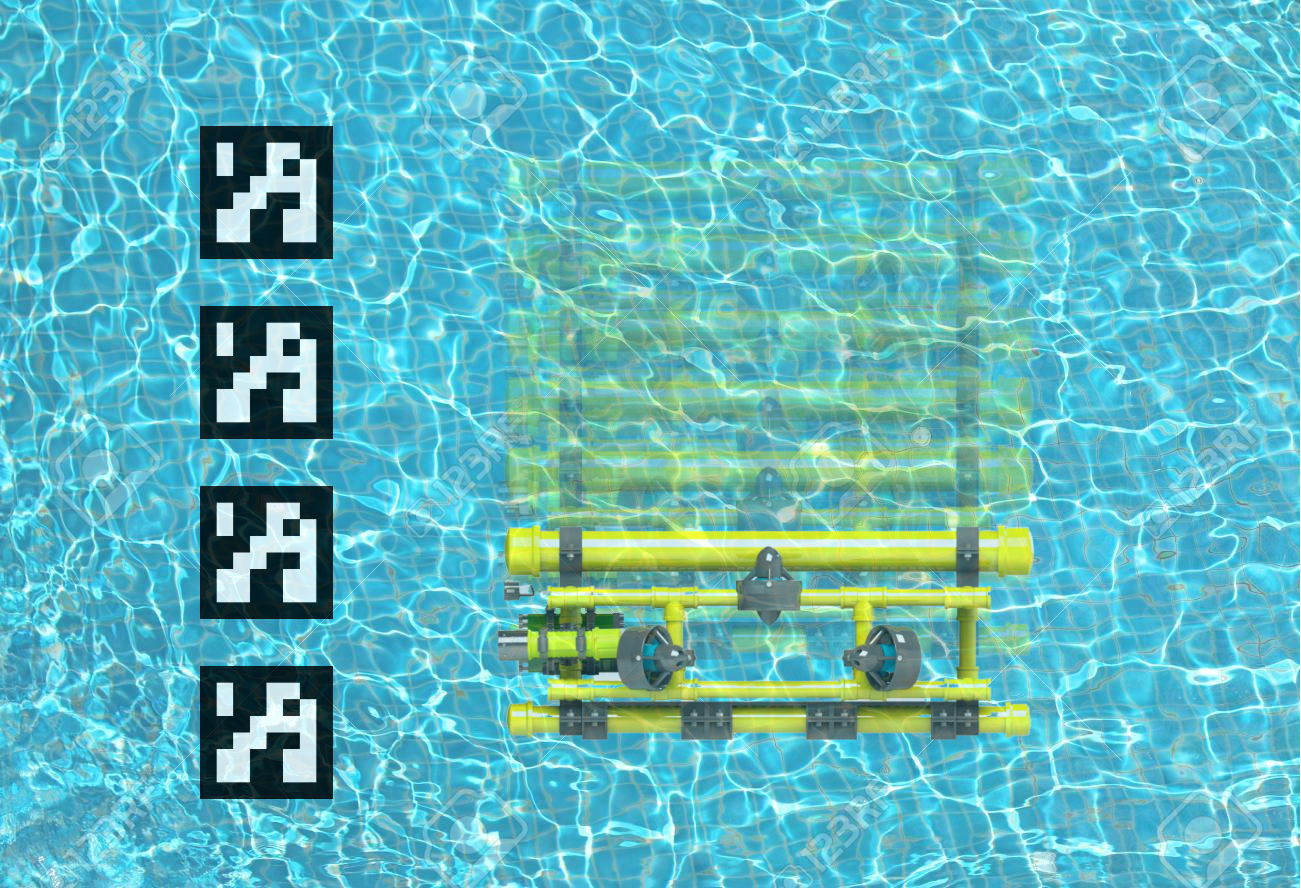
\includegraphics[width=0.8\linewidth]{images/descent_test}\\
	\footnotesize Fonte: Autores
\end{figure}


Dessa forma, os requisitos 2, 6 e 7 (apresentados na Seção \ref{sec:metodologia}) seriam validados, visto que, para a execução dessa tarefa, o ROV deve ser capaz de ir para uma posição previamente conhecida, localizar os Arucos e submergir e emergir de forma controlada.

\subsubsection*{Teste de velocidade e trajetória circular}

O requisito 3 determina a velocidade máxima que o veículo deve atingir. Então, é necessário que haja algum teste em que os motores do veículo operem na máxima capacidade de modo a se verificar se a velocidade determinada pode ser alcançada. O ROV foi projetado para ter mais velocidade em \textit{surge}, de forma a se deslocar mais rápido ao se mover para frente. Nesse contexto, o teste de velocidade consiste em colocar a referência de velocidade no seu valor máximo e medir a velocidade de deslocamento do ROV nesse trecho, porém essa medição é pouco precisa com a configuração de sensores atuais.

Portanto, para medir a velocidade, serão posicionados Arucos de diferentes tamanhos e o sistema de SBL. A configuração do ambiente de teste pode ser observada na Figura \ref{fig:speedtest}. 

\begin{figure}[h]
	\centering
	\caption{Missão de velocidade máxima e seguimento de trajetória}
	\label{fig:speedtest}
	\includegraphics[width=0.8\linewidth]{images/speed_test}\\
	\footnotesize Fonte: Autores
\end{figure}

Outra missão que será executada nessa mesma configuração é a execução de uma trajetória circular, para validação dos requisitos 4, 6 e 7. Ao se executar a trajetória circular, mantendo-se a profundidade e mantendo-se os Arucos no campo de visão da câmera, pode-se usar o armazenamento da trajetória para validar se o requisito de seguir uma trajetória realmente foi cumprido.

\subsubsection*{Mapeamento de rampa}

A validação do requisito 5, que se refere ao mapeamento do leito marinho, pode ser
feito através da utilização de um terreno conhecido. Então, propõe-se aqui a execução do simples mapeamento de uma rampa. Caso a inclinação da rampa seja semelhante ao do mapeamento, pode-se afirmar que o sistema funciona. O mapeamento não será muito detalhado, visto que irá se adquirir somente informação de 4 pontos, medidos com sensores de distância ultrassom abaixo do ROV. Portanto, um cenário simples como uma rampa é adequado para validação. Além disso, também se necessita do Aruco para posicionamento do ROV, como mostra a Figura \ref{fig:mappingtest}.

\begin{figure}[h]
	\centering
	\caption{Missão de mapeamento}
	\label{fig:mappingtest}
	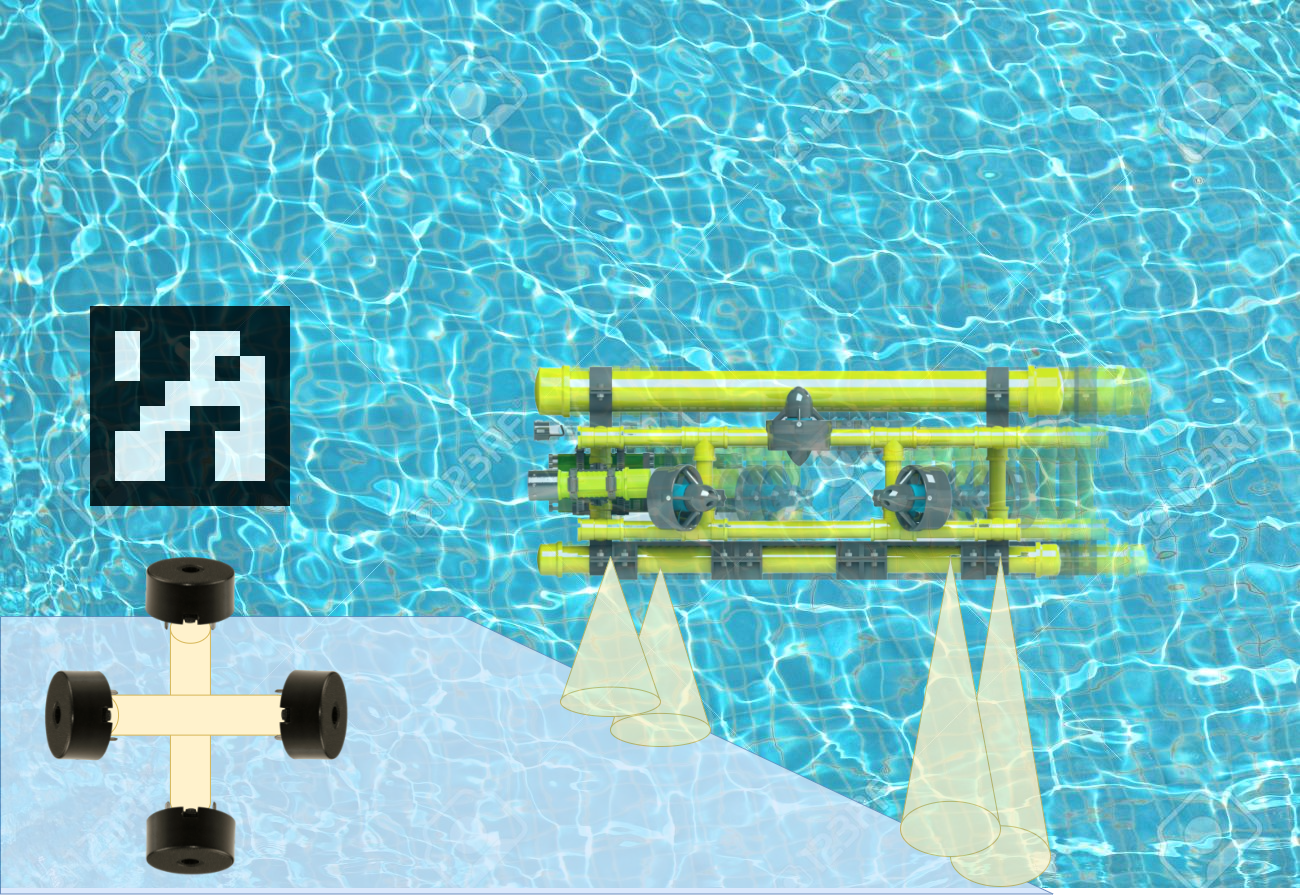
\includegraphics[width=0.8\linewidth]{images/mapping_test}\\
	\footnotesize Fonte: Autores
\end{figure}

\subsubsection*{Resgate da Moeda}
O requisito 8 determina que o ROV deve ser capaz de atender um pedido de socorro. Para a validação desse requisito, o BROV deve localizar a caixa de resgate, representada pelo aruco mais à esquerda da Figura \ref{fig:objectretrievingtest}. Além disso, deve esperar o led presente na caixa acender, para, a partir daí, se aproximar e capturar a moeda com seu imã e retornar a superfície. Esse teste não só valida o requisito 8, mas como todos os citados anteriormente. Para esse teste, tanto a localização por Aruco como a por SBL serão utilizados.

\begin{figure}[h]
	\centering
	\caption{Missão de resgate da moeda}
	\label{fig:objectretrievingtest}
	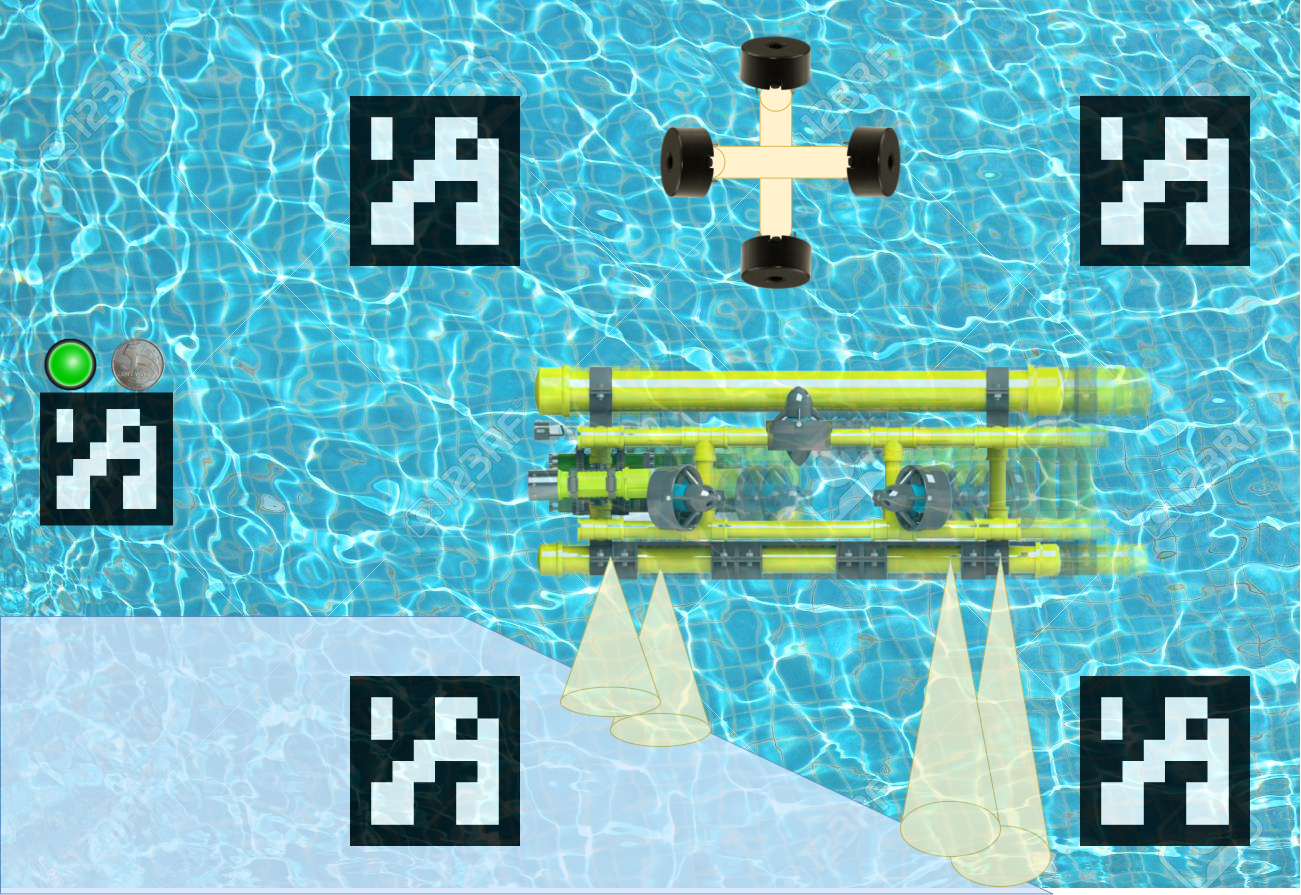
\includegraphics[width=0.8\linewidth]{images/object_retrieving_test}\\
	\footnotesize Fonte: Autores
\end{figure}


